\documentclass[12pt]{article}

\usepackage{geometry}
\geometry{textwidth=500pt,top=20mm,bottom=20mm}
\usepackage{pdflscape} % for landscape mode
\usepackage{longtable}
\usepackage{caption} % for captionsetup
\usepackage{graphicx}
\usepackage{hyperref}

\newcommand\MM{{\tt MulensModel}}


\begin{document} % ########################################

\begin{center}
%\centering

\includegraphics[width=0.5\textwidth]{logo/logoMM_crop_4_744x520.png}
\end{center}

\vspace*{3cm}

\begin{center}
{\LARGE Microlensing parameters in \MM}\\
\bigskip
Radek Poleski\\
last update: Apr 2024
\end{center}

\bigskip
Microlensing parameters in \MM\, class {\tt ModelParameters} are presented on the next page:

\begin{landscape}
\captionsetup{width=20cm}
\begin{longtable}{l l l p{12cm}}
Parameter & Name in \MM &  Unit & Description \\
\hline
$t_0$ & {\tt t\_0} & & The time of the closest approach between the source and the lens. \\
$u_0$ & {\tt u\_0} & & The impact parameter between the source and the lens center of mass. \\
$t_{\rm E}$ & {\tt t\_E} & d & The Einstein crossing time. \\
$t_{\rm eff}$ & {\tt t\_eff} & d & The effective timescale, $t_{\rm eff} \equiv u_0 t_{\rm E}$. \\
$\rho$ & {\tt rho} & & The radius of the source as a fraction of the Einstein ring. \\
$t_{\star}$ & {\tt t\_star} & d & The source self-crossing time, $t_\star \equiv \rho t_{\rm E}$. \\
$\pi_{{\rm E}, N}$ & {\tt pi\_E\_N} & & The North component of the microlensing parallax vector. \\
$\pi_{{\rm E}, E}$ & {\tt pi\_E\_E} & & The East component of the microlensing parallax vector. \\
$t_{0,{\rm par}}$ & {\tt t\_0\_par} & & The reference time for parameters in parallax models.$^a$ \\
$K$ & {\tt convergence\_K} & & External mass sheet convergence. \\
$G$ & {\tt shear\_G} & & External mass sheet shear; complex valued to represent both the magnitude and angle relative to the binary axis. \\
$s$ & {\tt s} & & The projected separation between the lens primary and its companion as a fraction of the Einstein ring radius. \\
$q$ & {\tt q} & & The mass ratio between the lens companion and the lens primary $q \equiv m_2/m_1$. \\
$\alpha$ & {\tt alpha} & deg. & The angle between the source trajectory and the binary axis. \\
$ds/dt$ & {\tt ds\_dt} & yr$^{-1}$ & The rate of change of the separation. \\
$d\alpha/dt$ & {\tt dalpha\_dt} & deg.~yr$^{-1}$ & The rate of change of $\alpha$. \\
$s_{z}$ & {\tt s\_z} & & Separation along the line of sight as a fraction of the Einstein ring radius. Positive axis points to the observer. \\
$ds_{z}/dt$ & {\tt ds\_z\_dt} & yr$^{-1}$ & The rate of change of the separation $s_{z}$. \\
$t_{0,{\rm kep}}$ & {\tt t\_0\_kep} & & The reference time for lens orbital motion calculations.$^a$ \\
$x_{\rm caustic, in}$ & {\tt x\_caustic\_in} & & Curvelinear coordinate of caustic entrance for a binary lens model.$^b$ \\
$x_{\rm caustic, out}$ & {\tt x\_caustic\_out} & & Curvelinear coordinate of caustic exit for a binary lens model.$^b$ \\
$t_{\rm caustic, in}$ & {\tt t\_caustic\_in} & & Epoch of caustic exit for a binary lens model.$^b$ \\
$t_{\rm caustic, out}$ & {\tt t\_caustic\_out} & & Epoch of caustic exit for a binary lens model.$^b$ \\
$\xi_P$ & \texttt{xi\_period} & d & The orbital period of xallarap.\\
$\xi_a$ & \texttt{xi\_semimajor\_axis} & & The semimajor axis of a xallarap orbit as a fraction of the Einstein ring.\\
$\xi_i$ & \texttt{xi\_inclination} & deg & The inclination of a xallarap orbit.$^c$\\
$\xi_\Omega$ & \texttt{xi\_Omega\_node} & deg & The longitude of the ascending node of a xallarap orbit.$^c$\\
$\xi_u$ & \texttt{xi\_argument\_of\_latitude\_reference} & deg & The argument of latitude at the reference epoch ($t_{0,\chi}$). The argument of latitude is a sum of true anomaly ($\nu$, changes with time) and the argument of periapsis ($\omega$, orbit parameter, i.e., does not change with time): $u = \nu + \omega$.$^c$\\
$\xi_e$ & \texttt{xi\_eccentricity} & & The eccentricity of a xallarap orbit.\\
$\xi_\omega$ & \texttt{xi\_omega\_periapsis} & deg & The argument of periapsis of a xallarap orbit.$^c$\\
$q_\mathrm{source}$ & \texttt{q\_source} & & Mass ratio of source components: $m_{s,2}/m_{s,1}$. It is valid only for xallarap models.\\
$t_{0,\xi}$ & \texttt{t\_0\_xi} & &  The reference epoch for parameters in xallarap models.$^a$\\
\hline
\caption{Notes: \newline
$^a$ -- $t_{0,{\rm par}}$, $t_{0,{\rm kep}}$, and $t_{0,\chi}$ are reference parameters, hence, do not change these during fitting. \newline
$^b$ -- The four parameters of binary lens in Cassan (2008) parameterization ($x_{\rm caustic, in}$, $x_{\rm caustic, out}$, $t_{\rm caustic, in}$, $t_{\rm caustic, out}$) are used instead of ($t_0$, $u_0$, $t_{\rm E}$, $\alpha$). \newline
$^c$ -- The orbital angles are illustrated in Figure~1.
%\label{}
}
\end{longtable}
\end{landscape}

Some of the parameters can be defined separately for each of the sources in binary source models.  
In that case, add {\tt \_1} or {\tt \_2} to parameter name. These are:
\begin{itemize}
\item {\tt t\_0\_1}, {\tt t\_0\_2},
\item {\tt u\_0\_1}, {\tt u\_0\_2},
\item {\tt rho\_1}, {\tt rho\_2},
\item {\tt t\_star\_1}, {\tt t\_star\_2}.
\end{itemize}

Also note that there are properties of the microlensing events that are not considered parameters in the \texttt{ModelParameters} class, but are implemented in other parts of the \texttt{MulensModel}. The most important are:
\begin{itemize}
 \item source and blending fluxes -- \texttt{Event} and \texttt{FitData}; also see use case 38,
 \item sky coordinates -- \texttt{Model.coords},
 \item limb-darkening coefficients -- \texttt{Model.set\_limb\_coeff\_gamma} and \texttt{Model.set\_limb\_coeff\_u},
 \item flux ratio for binary source models -- \texttt{Model.set\_source\_flux\_ratio} and\\ \texttt{Model.set\_source\_flux\_ratio\_for\_band},
 \item methods used to calculate magnification -- \texttt{Model.set\_magnification\_methods},
 \item coordinates of space telescopes -- \texttt{Model.get\_satellite\_coords}.
\end{itemize}

\begin{figure}
\centering
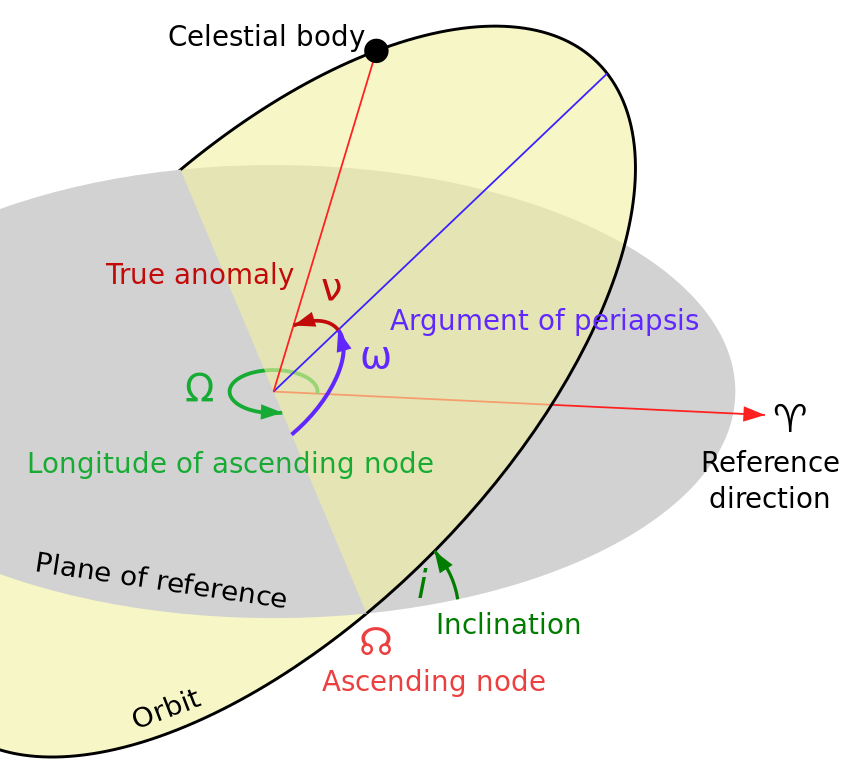
\includegraphics[width=0.56\textwidth]{images/orbit_parameters/Orbit1_svg}
\rotatebox[origin=l]{90}{\tiny image by Lasunncty/WikiCommons, license: CC BY-SA 3.0}
\caption{
Definition of orbital angles. 
There are Wikipedia articles that give more details: 
\href{https://en.wikipedia.org/wiki/Orbital_elements}{orbital elements} and 
\href{https://en.wikipedia.org/wiki/Argument_of_latitude}{argument of latitude}.
For xallarap, the reference direction is the relative lens-source proper motion direction and the reference plane is the plane of the sky. 
}
\end{figure}

\end{document}

